\documentclass[honours,12pt,twoside]{unswthesis}

\usepackage{afterpage}
\usepackage{amsfonts}
\usepackage{amsmath}
\usepackage{amssymb}
\usepackage{amsthm}
\usepackage[english]{babel}
\usepackage{graphicx}
\usepackage{natbib}
\usepackage[utf8]{inputenc}
\usepackage{latexsym}
\usepackage{url}
\usepackage{todonotes}
\usepackage{tikz}
\usepackage{pdfpages}
\usetikzlibrary{arrows}
\usepackage{float}
\usepackage[algoruled,boxed,lined]{algorithm2e}

\usepackage{booktabs}
\renewcommand{\arraystretch}{1.2}


%%%%%%%%%%%%%%%%%%%%%%%%%%%%%%%%%%%%%%%%%%%%%%%%%%%%%%%%%%%%%%%%%
%
%  The following are some simple LaTeX macros to give some
%  commonly used letters in funny fonts. You may need more or less of
%  these
%
\newcommand{\R}{\mathbb{R}}
\newcommand{\Q}{\mathbb{Q}}
\newcommand{\C}{\mathbb{C}}
\newcommand{\N}{\mathbb{N}}
\newcommand{\F}{\mathbb{F}}
\newcommand{\PP}{\mathbb{P}}
\newcommand{\T}{\mathbb{T}}
\newcommand{\Z}{\mathbb{Z}}
\newcommand{\B}{\mathfrak{B}}
\newcommand{\BB}{\mathcal{B}}
\newcommand{\M}{\mathfrak{M}}
\newcommand{\X}{\mathfrak{X}}
\newcommand{\Y}{\mathfrak{Y}}
\newcommand{\CC}{\mathcal{C}}
\newcommand{\E}{\mathbb{E}}
\newcommand{\cP}{\mathcal{P}}
\newcommand{\cS}{\mathcal{S}}
\newcommand{\A}{\mathcal{A}}
\newcommand{\ZZ}{\mathcal{Z}}

%%%%%%%%%%%%%%%%%%%%%%%%%%%%%%%%%%%%%%%%%%%%%%%%%%%%%%%%%%%%%%%%%%%%%
%
% The following are much more esoteric commands that I have left in
% so that this file still processes. Use or delete as you see fit
%
\newcommand{\bv}[1]{\mbox{BV($#1$)}}
\newcommand{\comb}[2]{\left(\!\!\!\begin{array}{c}#1\\#2\end{array}\!\!\!\right)
}
\newcommand{\Lat}{{\rm Lat}}
\newcommand{\var}{\mathop{\rm var}}
\newcommand{\Pt}{{\mathcal P}}
\def\tr(#1){{\rm trace}(#1)}
\def\Exp(#1){{\mathbb E}(#1)}
\def\Exps(#1){{\mathbb E}\sparen(#1)}
\newcommand{\floor}[1]{\left\lfloor #1 \right\rfloor}
\newcommand{\ceil}[1]{\left\lceil #1 \right\rceil}
\newcommand{\hatt}[1]{\widehat #1}
\newcommand{\modeq}[3]{#1 \equiv #2 \,(\text{mod}\, #3)}
\newcommand{\rmod}{\,\mathrm{mod}\,}
\newcommand{\p}{\hphantom{+}}
\newcommand{\vect}[1]{\mbox{\boldmath $ #1 $}}
\newcommand{\reff}[2]{\ref{#1}.\ref{#2}}
\newcommand{\psum}[2]{\sum_{#1}^{#2}\!\!\!'\,\,}
\newcommand{\bin}[2]{\left( \begin{array}{@{}c@{}}
				#1 \\ #2
			\end{array}\right)	}
%
%  Macros - some of these are in plain TeX (gasp!)
%
\newcommand{\be}{($\beta$)}
\newcommand{\eqp}{\mathrel{{=}_p}}
\newcommand{\ltp}{\mathrel{{\prec}_p}}
\newcommand{\lep}{\mathrel{{\preceq}_p}}
\def\brack#1{\left \{ #1 \right \}}
\def\bul{$\bullet$\ }
\def\cl{{\rm cl}}
\let\del=\partial
\def\enditem{\par\smallskip\noindent}
\def\implies{\Rightarrow}
\def\inpr#1,#2{\t \hbox{\langle #1 , #2 \rangle} \t}
\def\ip<#1,#2>{\langle #1,#2 \rangle}
\def\lp{\ell^p}
\def\maxb#1{\max \brack{#1}}
\def\minb#1{\min \brack{#1}}
\def\mod#1{\left \vert #1 \right \vert}
\def\norm#1{\left \Vert #1 \right \Vert}
\def\paren(#1){\left( #1 \right)}
\def\qed{\hfill \hbox{$\Box$} \smallskip}
\def\sbrack#1{\Bigl \{ #1 \Bigr \} }
\def\ssbrack#1{ \{ #1 \} }
\def\smod#1{\Bigl \vert #1 \Bigr \vert}
\def\smmod#1{\bigl \vert #1 \bigr \vert}
\def\ssmod#1{\vert #1 \vert}
\def\sspmod#1{\vert\, #1 \, \vert}
\def\snorm#1{\Bigl \Vert #1 \Bigr \Vert}
\def\ssnorm#1{\Vert #1 \Vert}
\def\sparen(#1){\Bigl ( #1 \Bigr )}

\newcommand\blankpage{%
    \null
    \thispagestyle{empty}%
    \addtocounter{page}{-1}%
    \newpage}
    
%%%%%%%%%%%%%%%%%%%%%%%%%%%%%%%%%%%%%%%%%%%%%%%%%%%%%%%%%%%%%%
%
% These environments allow you to get nice numbered headings
%  for your Theorems, Definitions etc.  
%
%  Environments
%
%%%%%%%%%%%%%%%%%%%%%%%%%%%%%%%
\newtheorem{theorem}{Theorem}[section]
\newtheorem{lemma}[theorem]{Lemma}
\newtheorem{proposition}[theorem]{Proposition}
\newtheorem{corollary}[theorem]{Corollary}
\newtheorem{conjecture}[theorem]{Conjecture}
%\theoremstyle{definition}
\newtheorem{definition}[theorem]{Definition}
\newtheorem{example}{Example}
\newtheorem{remark}[theorem]{Remark}
\newtheorem{question}[theorem]{Question}
\newtheorem{notation}[theorem]{Notation}
\numberwithin{equation}{section}

\begin{document}

\chapter{Neural networks}\label{neuralNets-intro}

This chapter outlines the structure and workings of basic neural network models. Those who have a basic understanding of neural networks and wish to avoid the details surrounding model structure and minimisation algorithms can proceed to Chapter \ref{convnets} for an overview of convolutional neural networks and Chapter \ref{litrev} for existing lacune model attempts.

% - Basic neural networks theory + perceptron
% - Loss functions
% - Minimisation functions
% 
% - Convolutional neural networks overview
% - Convolution layer
% - ReLU
% - Pooling
% - Fully connected layers
% 
% - 3D CNNs overview

Neural networks have become increasingly popular with advances in computing power and the availability of large data sets \cite{Goodfellow-et-al-2016}. They have been proven successful with \textsc{mri} discrimination tasks \cite{DouQ.2016ADoC, Yokoyama2007} and image classification tasks \cite{HeKaiming2015DDiR, AlexNet2012, GoogLeNet2015}. In some instances, neural networks have exhibited a higher image recognition accuracy than humans \cite{HeKaiming2015DDiR}.

The construction of neural networks has to be conducted with care. The resulting models are difficult to interpret and prone to overfitting. We now discuss the underlying structure of neural networks, loss minimisation, and techniques to avoid overfitting the data.

\section{Basic structure}\label{nnets-structure}

The structure of neural networks are analogous to that of neurons in the brain. Each brain cell receives a signal, conducts a small amount of processing, and passes the resulting signal to the next cell. Decisions made by the brain are the result of many neurons processing information in sequence. Neural networks adopt a similar structure. Individual nodes receive variables, apply a transformation, and pass the result to the next node. For this reason, the nodes are referred to as \textit{neurons}.

The structure of a neural network neuron is shown in Figure \ref{nnet-neuronfig}. Let $\mathbf{x} = (x_1, x_2, \ldots, x_n)^\intercal$ be a vector of $n$ input variables. Let $\mathbf{w} = (w_1, \ldots, w_n)^\intercal$ be a vector of weights. Let $b$ be an additional \textit{bias} variable. This bias is not to be confused with statistical bias and is included to provide the neuron with a constant term. This additional weight can be used to leverage the value of the neuron just before output, independent of the input variables. The output of a single neuron is given by
\begin{align}
	a = \sigma(\mathbf{w}\cdot\mathbf{x} + b),
\end{align}
where $\sigma(\cdot)$ is some function known as an \textit{activation function} and $a$ is an \textit{activation value}.



% Neuron structure diagram
\begin{figure}
\centering
\tikzset{every picture/.style={line width=0.75pt}} %set default line width to 0.75pt        

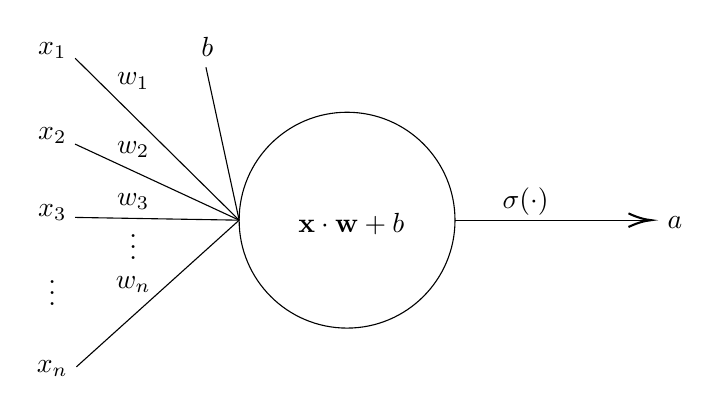
\begin{tikzpicture}[x=0.75pt,y=0.75pt,yscale=-1,xscale=1]
%uncomment if require: \path (0,300); %set diagram left start at 0, and has height of 300

%Shape: Circle [id:dp7806506925261892] 
\draw   (270,154) .. controls (270,125.28) and (293.28,102) .. (322,102) .. controls (350.72,102) and (374,125.28) .. (374,154) .. controls (374,182.72) and (350.72,206) .. (322,206) .. controls (293.28,206) and (270,182.72) .. (270,154) -- cycle ;
%Straight Lines [id:da48045113953293783] 
\draw    (191,76) -- (270,154) ;


%Straight Lines [id:da20730706323067383] 
\draw    (190.92,117.33) -- (270,154) ;


%Straight Lines [id:da19390293965519045] 
\draw    (191.59,224.67) -- (270,154) ;


%Straight Lines [id:da5499170807272789] 
\draw    (374,154) -- (466.51,154) ;
\draw [shift={(468.51,154)}, rotate = 180] [color={rgb, 255:red, 0; green, 0; blue, 0 }  ][line width=0.75]    (10.93,-3.29) .. controls (6.95,-1.4) and (3.31,-0.3) .. (0,0) .. controls (3.31,0.3) and (6.95,1.4) .. (10.93,3.29)   ;

%Straight Lines [id:da7426731370805287] 
\draw    (270,154) -- (190.92,152.67) ;


%Straight Lines [id:da35133187079282135] 
\draw    (254,80.33) -- (270,154) ;

% Text Node
\draw (324,156) node   {$\mathbf{x} \cdot \mathbf{w} +b$};
% Text Node
\draw (180,72.33) node   {$x_{1}$};
% Text Node
\draw (180,113.33) node   {$x_{2}$};
% Text Node
\draw (180,185) node   {$\vdots $};
% Text Node
\draw (180,225.33) node   {$x_{n}$};
% Text Node
\draw (180,150.33) node   {$x_{3}$};
% Text Node
\draw (219,87) node   {$w_{1}$};
% Text Node
\draw (219,120) node   {$w_{2}$};
% Text Node
\draw (219,145) node   {$w_{3}$};
% Text Node
\draw (219,185) node   {$w_{n}$};
% Text Node
\draw (219,163) node   {$\vdots $};
% Text Node
\draw (254.67,70.33) node   {$b$};
% Text Node
\draw (408,145) node   {$\sigma ( \cdot )$};
% Text Node
\draw (480,155) node   {$a$};


\end{tikzpicture}
\caption{Neuron structure.}
\label{nnet-neuronfig}
\end{figure}

%% Diagram of single neuron
%\begin{figure}[ht]
%	\centering
%	\includegraphics[scale=0.5]{Images/3_neuron.png}
%	\caption{Neuron structure.}
%	\label{nnet-neuronfig}
%\end{figure}

\begin{example}
\label{nnets-and-eg}
A logical \textsc{and} gate of two inputs can be expressed as a neuron. Let \textsc{true} be encoded to 1 and \textsc{false} be encoded to 0, so that $x_i \in \{0,1\}$ for $i=1,2$. Let $\mathbf{w} = (1, 1)^\intercal$ and $b = -1.5$. Let the activation function to be the step function $\sigma(z) = 1$ for $z > 0$ and $\sigma(z) = 0$ otherwise. The resulting neuron has output
\begin{align}
	a(\mathbf{x}) = \begin{cases}
		1 & x_1 + x_2 - 1.5 > 0\\
		0 & otherwise
	\end{cases},
\end{align}
which will output 1 only when $\mathbf{x} = (1, 1)^\intercal$.
\end{example}


A large number of these neurons can be arranged to form a neural network. The generated outputs of these neurons can be fed as inputs into later neurons. Basic neural networks arrange a number of these neurons into layers, as shown in Figure \ref{nnet-structurefig}. The first layer is an input layer, where data is fed into the model. Each neuron in this first layer represents a variable. The last layer is an output layer which generates the final result. The central layers, which conduct most of the processing, are known as \textit{hidden layers} and are shown as Hidden layer 1 and Hidden layer 2 in Figure \ref{nnet-structurefig}.

% Diagram of basic neural network structure. Input, 1 hidden layer and series of output layers
%\begin{figure}[ht]
%	\centering
%	\includegraphics[width=\textwidth]{Images/3_nnet_structure.jpg}
%	\caption{Basic neural network structure.}
%	\small Image taken from \url{`https://www.digitaltrends.com/cool-tech/what-is-an-artificial-neural-network/'}
%	\label{nnet-structurefig}
%\end{figure}
\begin{figure}
\centering
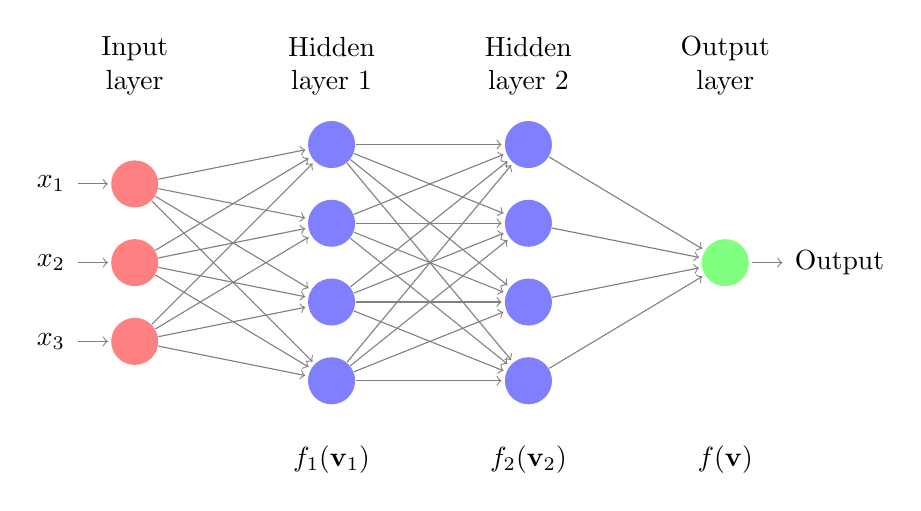
\begin{tikzpicture}[shorten >=1pt,->,draw=black!50, node distance=\layersep]
    \tikzstyle{every pin edge}=[<-,shorten <=1pt]
    \tikzstyle{neuron}=[circle,fill=black!25,minimum size=17pt,inner sep=0pt]
    \tikzstyle{input neuron}=[neuron, fill=red!50];
    \tikzstyle{output neuron}=[neuron, fill=green!50];
    \tikzstyle{hidden neuron}=[neuron, fill=blue!50];
    \tikzstyle{annot} = [text width=4em, text centered]
	\def\layersep{2.5cm}
	
    % Draw the input layer nodes
    \foreach \name / \y in {1,...,3}
    % This is the same as writing \foreach \name / \y in {1/1,2/2,3/3,4/4}
        \node[input neuron, pin=left:$x_\y$] (I-\name) at (0,-\y) {};

    % Draw the hidden layer1 nodes
    \foreach \name / \y in {1,...,4}
        \path[yshift=0.5cm]
            node[hidden neuron] (Ha-\name) at (\layersep,-\y cm) {};
            
    % Draw the hidden layer2 nodes
    \foreach \name / \y in {1,...,4}
        \path[yshift=0.5cm]
            node[hidden neuron] (Hb-\name) at (2*\layersep,-\y cm) {};

    % Draw the output layer node
    \node[output neuron,pin={[pin edge={->}]right:Output}] (O) at (3*\layersep, -2) {};

    % Connect every node in the input layer with every node in the
    % hidden layer.
    \foreach \source in {1,...,3}
        \foreach \dest in {1,...,4}
            \path (I-\source) edge (Ha-\dest);
            
    % Connect every node in the hidden layer 1 with every node in
    % hidden layer 2.
    \foreach \source in {1,...,4}
        \foreach \dest in {1,...,4}
            \path (Ha-\source) edge (Hb-\dest);

    % Connect every node in the hidden layer with the output layer
    \foreach \source in {1,...,4}
        \path (Hb-\source) edge (O);

    % Annotate the layers
    \node[annot,above of=Ha-1, node distance=1cm] (hla) {Hidden layer 1};
    \node[annot,above of=Hb-1, node distance=1cm] (hlb) {Hidden layer 2};
    \node[annot,left of=hla] {Input layer};
    \node[annot,right of=hlb] {Output layer};
    
    \node[annot,below of=Ha-4, node distance=1cm] (fa) {$f_1(\mathbf{v}_1)$};
    \node[annot,below of=Hb-4, node distance=1cm] (fb) {$f_2(\mathbf{v}_2)$};
    \node[annot,right of=fb, node distance=\layersep] (fo) {$f(\mathbf{v})$};

\end{tikzpicture}
\caption{Basic neural network structure. Each hidden neuron (blue) and the output neuron (green) has the structure shown in Figure \ref{nnet-neuronfig}. For simplicity, the weights and biases have been hidden.}
\label{nnet-structurefig}
\end{figure}

Let the weights and biases of the $\ell$-th layer be $\mathbf{v}_\ell$ and let the output of hidden layer $\ell$ be $f_\ell(\mathbf{v}_\ell)$. Then the output of the whole network is
\begin{align}
	f(\mathbf{v}) = f_L(\mathbf{v}_L) \circ f_{L-1}(\mathbf{v}_{L-1}) \circ \cdots \circ f_1(\mathbf{v}_1).
\end{align}

During model fitting, the quality of the model is quantified using some \textit{cost function} $C(W,B)$, where a cost of 0 describes a perfect model fit. The set of weights $W$ and set of biases $B$ are trained to minimise this cost function with respect to $(W,B)$. However, since the number of variables can be very large, it is not always feasible to analytically minimise $C(W,B)$. Instead, we can approximate this minimisation via the Gradient-Descent algorithm (see Section \ref{nnets-graddesc}). This algorithm is repeated until the cost function falls within some tolerance $\tau$, or reaches the maximum number of iterations $n_T$.

\section{Notation}\label{nnets-not}



\begin{tabular}{p{1cm}p{13cm}}
$\mathbf{a}^\ell$ & vector of activation values (outputs) of the $\ell$-th layer.\\
$a_j^\ell$ & $j$-th element of $\mathbf{a}^\ell$, the activation value of the $j$-th neuron of the $\ell$-th layer.\\
$\mathbf{w}^\ell$ & matrix of weights used to compute the vector $\mathbf{a}^\ell$.\\
$\mathbf{w}^\ell_j$ & vector of weights used to compute $a_j^\ell$.\\
$w_{ji}^\ell$ & $i$-th element of $\mathbf{w}^\ell_j$, to be multiplied with $a_i^{\ell-1}$.\\
$b_j^\ell$ & bias of the $j$-th neuron of the $\ell$-th layer.\\
$z_j^\ell$ & $:= \mathbf{w}_j^\ell\cdot \mathbf{a}^{\ell-1} + b_j^\ell= \sum_k w_{jk}^\ell a_k^{\ell-1} + b_j^\ell$. The value of the $j$-th neuron of the $\ell$-th layer before the activation function $\sigma(\cdot)$ is applied.\\
$\mathbf{z}^\ell$ & vector of $z_j^\ell$ of the $\ell$-th layer.\\
$\delta_j^\ell$ & $:=\dfrac{\partial C}{\partial z_j^\ell}$. The gradient error in the $j$-th neuron of the $\ell$-th layer when minimising the cost function $C$.\\
$\delta^\ell$ & Vector of errors $\delta_j^\ell$ for the $\ell$-th layer.\\
$Z$ & set of all $z_j^\ell$ in the network. \\
$W$ & set of all weights $w_{jk}^\ell$ in the network.\\
$B$ & set of all biases $b_j^\ell$ in the network. \\
$\mathbf{v}$ & $:= (W,B)$. The set of all weights and biases.\\
$L$ & number of layers in the network.\\
$X$ & set of $n$ training inputs $\{\mathbf{x}_1, \mathbf{x}_2, \ldots, \mathbf{x}_n\}$. \\
$Y$ & set of $n$ training responses $\{\mathbf{y}_1, \mathbf{y}_2, \ldots, \mathbf{y}_n\}$.\\
$\eta$ & learning rate, controls the magnitude of adjustments made to weights during training.
\end{tabular}

%Let $\mathbf{w}^\ell_j$ to be the vector of weights used to compute the $j$-th neuron of the $\ell$-th layer, where $w_{ji}^\ell$ is the weight attributed to the $i$-th neuron of the $(\ell-1)$-th layer.

%Let $b_j^\ell$ be the bias of the $j$-th neuron in the $\ell$-th layer.

%Let $\mathbf{a}^\ell$ be the vector of activation values (outputs) for the $\ell$-th layer, where $a_j^\ell$ is the activation value of the $j$-th neuron of that layer. Set $z_j^\ell := \mathbf{w}_j^\ell\cdot \mathbf{a}^{\ell-1} + b_j^\ell= \sum_k w_{jk}^\ell a_k^{\ell-1} + b_j^\ell$ to be the values calculated before activation, and $\mathbf{z}^\ell$ to be the vector of $z_j^\ell$ for the $\ell$-th layer. 
%Set $Z$ to be the set of all $z_j^\ell$ in the whole network. 
%Let $L$ be the number of layers in the network so that $\mathbf{a}^L$ is the vector of activation values of the final output layer. 
%Let $X = \{\mathbf{x}_1, \mathbf{x}_2, \ldots, \mathbf{x}_n\}$ be the set of $n$ training inputs. 
%Let the responses be $Y = \{\mathbf{y}_1, \mathbf{y}_2, \ldots, \mathbf{y}_n\}$, with $y_{ij}$ the $j$-th variable of $\mathbf{y}_i$. 
%Let $W$ and $B$ be the sets of all weights and biases as before. Let $\eta$ be the learning rate of the network. 
\pagebreak
\section{Activation functions}\label{nnets-act}

Activation functions, denoted by $\sigma(\cdot)$, are applied just before neuron output. Without these functions, the network can be reduced to a linear combination of inputs. Activation functions avoid this by introducing nonlinearity into the model.

The simplest neuron type is the \textit{perceptron}, used in Example \ref{nnets-and-eg}. It is characterised by,
\begin{align}
	x_i \in \{0,1\} \text{ and } \sigma(z) = \begin{cases}
		1 & z > 0 \\
		0 & z \le 0
	\end{cases}.
\end{align}

To allow for continuous outputs, other common activation functions include the sigmoids, which are monotonically increasing, smooth approximations to the step function. Examples of these include the sigmoid function
\begin{align}
	\sigma(z) = \dfrac{1}{1+e^{-z}},
\end{align}
and hyperbolic tan function
\begin{align}
	\sigma(z) = \tanh(z).
\end{align}
Both the sigmoid and hyperbolic tan functions are common activation functions \cite{Goodfellow-et-al-2016}, however they are computationally expensive and so are not preferred for image recognition tasks as they contain a large number of variables \cite{LeCun2012, Nielson2015}.

The Rectified Linear Unit (ReLU) activation is given by,
\begin{align}
	\sigma(z) = \max(0, z).
\end{align}
The ReLU activation function is suitable for neural network optimisation as the function and its derivative are simplistic \cite{Goodfellow-et-al-2016}. The neuron is said to be \textit{active} for $z > 0$. In this region, the gradient is constant and large for positive input values, promoting training of the neuron's weights (see Section \ref{nnets-graddesc} on Gradient Descent). For $z \leq 0$, the neuron has a gradient of 0 and is deactivated, avoiding unnecessary parameter adjustments and computation. 

The softmax activation function,
\begin{align}
	\sigma(z_j) = \dfrac{e^{z_j}}{\sum_ke^{z_k}},
\end{align}
is used to structure the output layer as a discrete probability distribution over $k$ classes.


\section{Cost functions}\label{nnets-cost}

Weights and biases are chosen such that they approximately minimise some cost function. Nielson \cite{Nielson2015} describes two restrictions on cost functions for them to be minimised using the Gradient Descent algorithm (see Section \ref{nnets-graddesc}). The first requirement is that the cost $C_X(\cdot)$ accrued from all samples $X$ equals the mean of costs accrued from $n$ distinct subsamples of $X$, denoted by $X_i$,
\begin{align}
	C_X(W, B) = \dfrac{1}{n}\sum_{i=1}^n C_{X_i}(W,B).
\end{align}

The second requirement is that the cost is independent of $\mathbf{a}^\ell$ for all $\ell < L$. There are a number of cost functions in frequent use, and the choice of cost function depends on the structure of the response. A common cost function for regression is the \textit{quadratic cost}, or Mean Squared Error (\textsc{mse}) cost \cite{Nielson2015}. Denote $\|\cdot\|$ to be the Euclidean norm. The \textsc{mse} cost function is given by
\begin{align}
	C(W,B) = \dfrac{1}{2n}\sum_{i=1}^n||\mathbf{a}^L(\mathbf{x}_i,W,B) - \mathbf{y}_i ||^2.
\end{align}
This form is convenient for backpropagation (see Section \ref{nnets-backprop}) as it has an efficiently computable gradient,
\begin{align}
	\nabla_aC(W,B) = \dfrac{1}{n}\sum_{i=1}^n||\mathbf{a}^L(\mathbf{x}_i,W,B) - \mathbf{y}_i ||,
\end{align}
where $\nabla C(\mathbf{v}) = \Big(\dfrac{\partial C}{\partial v_1}, \dfrac{\partial C}{\partial v_2},\ldots, \dfrac{\partial C}{\partial v_N}\Big)$.
%In using quadratic cost, if the amount of error is large, the learning rate is low.

The most common cost function for classification tasks is \textit{cross-entropy} \cite{Nielson2015}, given by
\begin{align}\label{nnets-cross-entropy-eq}
	C(W,B) = -\dfrac{1}{n}\sum_{i=1}^n\sum_j\big[y_{ij}\log\big(a_j^L(\mathbf{x}_i,W,B)\big) + (1 - y_{ij})\log\big( (1 - a_j^L(\mathbf{x}_i,W,B))\big)\big],
\end{align}
with gradient
\begin{align}
	\nabla_aC(W,B) = \dfrac{1}{n}\sum_{i=1}^n\sum_j\dfrac{a_j^L(\mathbf{x}_i,W,B) - y_{ij}}{a_j^L(\mathbf{x}_i,W,B)(1-a_j^L(\mathbf{x}_i,W,B))}.
\end{align}

The efficacy of cross-entropy as a measure of misclassification cost can be shown through the Maximum Likelihood Estimator (\textsc{mle}) of the weights $(W, B)$ and also by considering distributional similarities between the data and the proposed model.

Let ${p}_{data}(\mathbf{x})$ be the unknown probability distribution of the data points $\mathbf{x}_1, \mathbf{x}_2, \ldots, \mathbf{x}_n$. Let $p_{model}(\mathbf{x}; \mathbf{\theta})$ be a family of probability distributions estimating the true $p_{data}(\mathbf{x})$. The \textsc{mle} of $\mathbf{\theta}$ is defined as
\begin{align}
	\hat{\mathbf{\theta}}_{MLE} = \arg\max_{\mathbf{\theta}}\prod_{i=1}^np_{model}(\mathbf{x}_i;\mathbf{\theta}).
\end{align}
This can be reformulated using the log-likelihood,
\begin{align}
	\hat{\mathbf{\theta}}_{MLE} = \arg\max_{\mathbf{\theta}}\sum_{i=1}^n\log p_{model}(\mathbf{x}_i;\mathbf{\theta}).
\end{align}
Dividing by $n$, the expression to be written in terms of expectation,
\begin{align}\label{nnets-mle-eq}
	\hat{\mathbf{\theta}}_{MLE} = \arg\max_{\mathbf{\theta}}\mathbb{E}_{\mathbf{x}\sim \hat{p}_{data}}\left[\log p_{model}(\mathbf{x}; \mathbf{\theta})\right].
\end{align}

\begin{definition}
	\textbf{Kullback-Leibler (KL)-divergence} is a measure of difference between two probability distributions $P(x)$ and $Q(x)$ given by
	\begin{align}
		D_{KL}(P||Q) = \mathbb{E}_{x\sim P}\left[\log\dfrac{P(x)}{Q(x)}\right] = \mathbb{E}_{x\sim P}[\log P(x) - \log Q(x)],
	\end{align}
	where $\cdot||\cdot$ denotes necessary ordering of the function inputs. Note that \textsc{kl}-divergence is not symmetric and is therefore not a metric.	
\end{definition}

Minimisation of the \textsc{kl}-divergence between $\hat{p}_{data}$ and $p_{model}$ is given by
\begin{align}\label{nnets-kl-eq}
	\hat{\theta}_{KL} = \arg\min_\theta\mathbb{E}_{\mathbf{x}\sim\hat{p}_{data}}\left[\log \hat{p}_{data}(\mathbf{x}) - \log p_{model}(\mathbf{x};\mathbf{\theta})\right].
\end{align}

Since $\hat{p}_{data}$ is not a function of $\mathbf{\theta}$, Equation \eqref{nnets-kl-eq} is equivalent to 
\begin{align}\label{nnets-kl-eq2}
	\hat\theta_{KL} = \arg\min_\theta-\mathbb{E}_{\mathbf{x}\sim\hat{p}_{data}}\left[\log p_{model}(\mathbf{x};\theta)\right].
\end{align}
Both the \textsc{mle} of $\theta$ (Equation \eqref{nnets-mle-eq}) and the minimiser of \textsc{kl}-divergence (Equation \eqref{nnets-kl-eq2}) are equivalent to the minimiser of cross-entropy (Equation \eqref{nnets-cross-entropy-eq}). 

% https://www.deeplearningbook.org/contents/ml.html P130
%The KL divergence between the empirical distribution $\hat{p}_{data}$ and 



%Unlike the quadratic cost, when the error is high, the learning rate is also high.

%Cost functions can include: the quadratic (simple), cross-entropy, regularisation (L1, L2, dropout, artificial expansion of training data).
%In using cross-entropy, the learning rate of the weight is controlled by the amount of error. This is unlike the quadratic cost function, which has a very slow learning rate when there is high error.
%Changing these can improve a model.
%Other improvements made by making better initialisations of weights, and better heuristics to choose hyper-parameters.

\section{The Gradient Descent algorithm}\label{nnets-graddesc}

Weights $W$ and biases $B$ are chosen such that they approximately minimise the cost function $C(W,B)$. Analytically minimising the cost function is possible, however the large number of variables makes this process slow, having time complexity $O(n^3)$ \cite{Marquardt1963}. The weights are instead estimated using the Gradient Descent algorithm, improving computation speed.

Gradient Descent considers the gradient of the cost given the current weights and biases \cite{Nielson2015}. The algorithm shifts the weights and biases by a small amount such that the cost decreases. The amount that the values are shifted by is referred to as the learning rate, denoted as $\eta$. Let $N$ be a positive integer and let $\mathbf{v} = (W,B)$. The approximate change in the cost function $C(\mathbf{v})$ as a result of the shifted $\mathbf{v}$ is given by the \textit{Total Differential Approximation}
\begin{align}
	\Delta C(\mathbf{v}) & \approx \dfrac{\partial C}{\partial v_1}\Delta v_1 + \dfrac{\partial C}{\partial v_2}\Delta v_2 + \cdots + \dfrac{\partial C}{\partial v_N}\Delta v_N\\
	& = \nabla C(\mathbf{v})\cdot \Delta \mathbf{v}.\label{nnets-total-diff-eq}
\end{align}


Define $\mathbf{v}':= \mathbf{v} + \Delta\mathbf{v}$ to be the updated value of $\mathbf{v}$. We update $\mathbf{v}'$ inductively such that the cost decreases by an amount proportional to $\eta$. At the next iteration, $\mathbf{v}$ is chosen such that the cost function decreases by an amount controlled by $\eta$, such that
\begin{align}
	\Delta\mathbf{v} = -\eta \nabla C(\mathbf{v}), \quad \text{ where }\eta > 0.
\end{align}
By substitution, Equation \eqref{nnets-total-diff-eq} can be written as
\begin{align}
	\Delta C(\mathbf{v}) \approx -\eta \|\nabla C(\mathbf{v})\|^2 \le 0.
\end{align}

Thus if $\mathbf{v}' := \mathbf{v} - \eta \nabla C(\mathbf{v})$, the cost function will decrease. In training a neural network, the size of the shift can be set to $\|\Delta\mathbf{v}\| = \varepsilon$, for some $\varepsilon > 0$. It can be shown that the $\Delta\mathbf{v}$ which gives the greatest decrease in $C(\mathbf{v})$ is a function of $\varepsilon$ and $\nabla C$ \cite{Nielson2015}.

\begin{lemma}\label{nnets-graddescminproof}
	Let $\varepsilon > 0$ and suppose the size of the shift is constrained such that $\|\Delta\mathbf{v}\| = \varepsilon$. Then $\nabla C \cdot \Delta\mathbf{v}$ is minimised by $\Delta\mathbf{v} = -\eta\nabla C$, where $\eta = \dfrac{\varepsilon}{\|\nabla C\|}$.
\end{lemma}

\begin{proof}
	By the Cauchy-Schwarz Inequality, we have
	\begin{align}
			|\nabla C\cdot\Delta\mathbf{v}| \le \|\nabla C\|\times\|\Delta\mathbf{v}\|.
	\end{align}
	The minimum is given by,
	\begin{align}\label{nnets-gdesc-eq1}
		\min(\nabla C\cdot\Delta\mathbf{v}) = -\|\nabla C\|\times\|\Delta\mathbf{v}\|.
	\end{align}
	Substituting $||\Delta\mathbf{v}|| = \epsilon$ into Equation 	\eqref{nnets-gdesc-eq1}, we have
	\begin{align}\label{nnets-gdesc-eq2}
		\min(\nabla C\cdot\Delta\mathbf{v}) = -\varepsilon\|\nabla C\|.
	\end{align}
	Multiplying the numerator and denominator of Equation \eqref{nnets-gdesc-eq2} by $||\nabla C||$ gives
	\begin{align}\label{nnets-gdesc-eq3}
		\min(\nabla C\cdot\Delta\mathbf{v}) & = -\dfrac{\varepsilon\|\nabla C\|^2}{\|\nabla C\|}\\[1em]
		& = -\dfrac{\varepsilon\nabla C\cdot\nabla C}{\|\nabla C\|} \label{nnets-gdesc-eq4}.
	\end{align}
	By equating the coefficients of $\nabla C$ between Equations \eqref{nnets-gdesc-eq1} and \eqref{nnets-gdesc-eq4}, and noting that $\eta = \epsilon / ||\nabla C||$,
	\begin{align}
		\operatorname*{arg\,min}_{\Delta\mathbf{v}}(\nabla C\cdot\Delta\mathbf{v}) & = -\dfrac{\varepsilon\nabla C}{\|\nabla C\|} \\
		& = -\eta\nabla C.
	\end{align}	
\end{proof}

The Gradient Descent algorithm moves the coefficients in the direction of the steepest negative gradient. It assumes that the starting values are close enough to the global minimum to converge. If this assumption is not satistifed, the algorithm will instead converge to the local minimum. In this thesis, we are only concerned about estimating the local minimum.

Since the updated weights and biases rely on the gradient, it should be noted that these gradients are required to be significantly different from zero. When this is not the case, the weights and biases stagnate and we have what is known as the Vanishing gradient problem, which is discussed further in Section \ref{nnet-vanishinggradprob}.

\subsection*{Stochastic Gradient Descent}\label{nnets-stochgraddesc}

Gradient Descent is a highly computationally intensive algorithm as the neural network has a very large number of weights. To improve training time, Stochastic Gradient Descent is a popular alternative as it has a time complexity $O(n)$ \cite{Robbins1951}. This algorithm improves learning speed by randomly selecting a small subset of the training set to learn from, referred to as a \textit{batch}. When training has been completed for that batch, a new batch of training inputs is randomly selected and the process repeats. Once training has occurred over all batches, it is said that an \textit{epoch} of training has been completed. In this manner, a relatively small number of samples is used for each weight adjustment. This drastically increases training speed whilst utilising all the information provided by the entire training set.

\subsection*{Learning rate}\label{nnets-learningrate}

During Gradient Descent, the change in gradients $\Delta\mathbf{v} = -\eta\nabla C$ moves the weights in the direction of the steepest negative gradient (see Section \ref{nnets-graddesc}). The learning rate $\eta$ controls the magnitude of the movement. If $\eta$ is too small, the adjustment of weights is also small and model training will take a long time. If $\eta$ is too large, the weights may be shifted too far and the values of $\mathbf{v}$ will continuously move past the local minimum. This is shown in Figure \ref{nnets-high-learn-fig}.

\begin{figure}[h]
\centering

\tikzset{every picture/.style={line width=0.75pt}} %set default line width to 0.75pt        

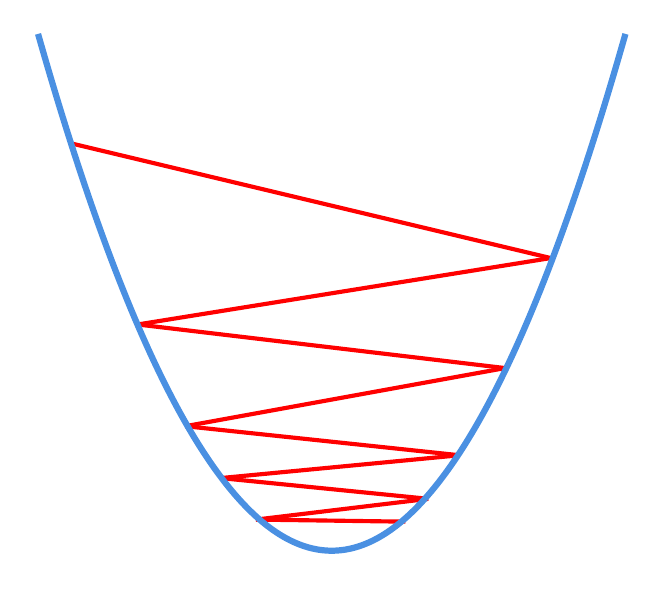
\begin{tikzpicture}[x=0.75pt,y=0.75pt,yscale=-1,xscale=1]
%uncomment if require: \path (0,291); %set diagram left start at 0, and has height of 291
\clip (85,15) rectangle (380,280);
%Straight Lines [id:da887590123175323] 
\draw [color={rgb, 255:red, 255; green, 0; blue, 0 }  ,draw opacity=1 ][line width=1.5]    (107,71) -- (337,126) ;


%Straight Lines [id:da9052100651701044] 
\draw [color={rgb, 255:red, 255; green, 0; blue, 0 }  ,draw opacity=1 ][line width=1.5]    (138,158) -- (337,126) ;


%Straight Lines [id:da30101863302529275] 
\draw [color={rgb, 255:red, 255; green, 0; blue, 0 }  ,draw opacity=1 ][line width=1.5]    (138,158) -- (315,179) ;


%Straight Lines [id:da06604062534938782] 
\draw [color={rgb, 255:red, 255; green, 0; blue, 0 }  ,draw opacity=1 ][line width=1.5]    (161,207) -- (315,179) ;


%Straight Lines [id:da6697786125314551] 
\draw [color={rgb, 255:red, 255; green, 0; blue, 0 }  ,draw opacity=1 ][line width=1.5]    (161,207) -- (293,221) ;


%Straight Lines [id:da4053203519455636] 
\draw [color={rgb, 255:red, 255; green, 0; blue, 0 }  ,draw opacity=1 ][line width=1.5]    (178,232) -- (293,221) ;


%Straight Lines [id:da553912866083977] 
\draw [color={rgb, 255:red, 255; green, 0; blue, 0 }  ,draw opacity=1 ][line width=1.5]    (178,232) -- (278,242) ;


%Straight Lines [id:da1577171267791595] 
\draw [color={rgb, 255:red, 255; green, 0; blue, 0 }  ,draw opacity=1 ][line width=1.5]    (195,252) -- (278,242) ;


%Straight Lines [id:da21468778984608516] 
\draw [color={rgb, 255:red, 255; green, 0; blue, 0 }  ,draw opacity=1 ][line width=1.5]    (195,252) -- (267,253) ;


%Shape: Parabola [id:dp09742535750627612] 
\draw  [color={rgb, 255:red, 74; green, 144; blue, 226 }  ,draw opacity=1 ][line width=2.25]  (90,18) .. controls (184.33,350) and (278.67,350) .. (373,18) ;

\end{tikzpicture}

\caption{High learning rates adjust weights past the local minimum}
\label{nnets-high-learn-fig}
\end{figure}

To aid in efficient training, learning rates can be adjusted throughout model training. At the start of training, it can be beneficial to have a higher learning rate. This allows the weights to move closer to the local minimum much faster. At later epochs, a smaller learning rate will allow for fine tuning of the weights, ensuring precision.

\subsection*{Adam Optimiser}\label{nnets-adam}

The Adam Optimiser is an algorithm that introduces additional learning rates to the Gradient Descent algorithm. Different learning rates are applied to each of the weights in the neural network, allowing the cost function to converge to the minimum more quickly \cite{Kingma2014}.


\section{The Backpropagation algorithm}\label{nnets-backprop}

During gradient descent, it is necessary to calculate the gradient of the cost function with respect to the weights $(W,B)$. The backpropagation algorithm is an efficient algorithm that determines $\dfrac{\partial C}{\partial z}$ and relates them to the rates of interest, $\dfrac{\partial C}{\partial W}$ and $\dfrac{\partial C}{\partial B}$ \cite{Nielson2015}. The following lemmas are necessary to understand the backpropagation algorithm.

% http://neuralnetworksanddeeplearning.com/chap2.html

\begin{lemma}
	The error of the $j$-th neuron of the final output layer is
	\begin{align}
		\delta_j^L = \dfrac{\partial C}{\partial a_j^L}\sigma'(z_j^L).
	\end{align}
	The vector of output layer errors can be expressed in the matrix form,
	\begin{align}\label{nnets-bprop-eq1}
		\delta^L = \Sigma'(\mathbf{z}^L)\nabla_aC,
	\end{align}
where $\Sigma'(\cdot)$ is a matrix such that the $j$-th diagonal entry is $\sigma'(z_j^L)$ and all non-diagonal entries are 0.
\end{lemma}

\begin{proof}

Since $z_j^L$ is only a function of $a_k^L$ for $k = j$, $\delta_j^L$ is
	\begin{align}
		\delta_j^L = \dfrac{\partial C}{\partial z_j^L} & = \sum_k\dfrac{\partial C}{\partial a_k^L}\dfrac{\partial a_k^L}{\partial z_j^L} \\
		& = \dfrac{\partial C}{\partial a_j^L}\dfrac{\partial a_j^L}{\partial z_j^L}\\
		& = \dfrac{\partial C}{\partial a_j^L}\sigma'(z_j^L).
	\end{align}
\end{proof}

\begin{lemma}
	The error $\delta^\ell_j$ of the $\ell$-th layer can be written in terms of the errors of the $(\ell + 1)$-th layer, 
	\begin{align}
		\delta_j^\ell & = \sum_k\delta_k^{\ell+1}w_{kj}^{\ell+1}\sigma'(z_j^\ell).
	\end{align}
	The vector of errors $\delta^\ell$ for the $\ell$-th layer can be expressed in the matrix form,
	\begin{align}\label{nnets-bprop-eq2}
		\delta^\ell & = \Sigma'(\mathbf{z}^\ell)(w^{\ell+1})^\intercal\delta^{\ell+1}
	\end{align}
		%& = \Sigma'(\mathbf{z}^\ell)(w^{\ell+1})^\intercal\cdots\Sigma'(\mathbf{z}^{L-1})(w^L)^\intercal\Sigma'(\mathbf{z}^L)\nabla_aC.
\end{lemma}

\begin{proof}
	Using the chain rule,
	\begin{align}
		\delta_j^\ell = \dfrac{\partial C}{\partial z_j^\ell}& = \sum_k\dfrac{\partial C}{\partial z_k^{\ell+1}}\dfrac{\partial z_k^{\ell+1}}{\partial z_j^\ell} \\
		& = \sum_k\delta_k^{\ell+1}\dfrac{\partial z_k^{\ell+1}}{\partial z_j^\ell}.
	\end{align}
	Since $\dfrac{\partial z_k^{\ell+1}}{\partial z_j^\ell} = \dfrac{\partial}{\partial z_j^\ell}(\mathbf{w}_k^{\ell+1}\cdot\sigma(\mathbf{z}^\ell) + b_k^{\ell+1}) = w_{kj}^{\ell+1}\sigma'(z_j^\ell)$, $\delta_j^\ell$ can be written
	\begin{align}
		\delta_j^\ell & = \sum_k\delta_k^{\ell+1}w_{kj}^{\ell+1}\sigma'(z_j^\ell).
	\end{align}
\end{proof}

\begin{lemma}
	The error $\delta_j^\ell$ is equivalent to the rate of change in the cost function with respect to the bias, such that
	\begin{align}\label{nnets-bprop-eq3}
		\delta_j^\ell = \dfrac{\partial C}{\partial b_j^\ell}.
	\end{align}
\end{lemma}
\begin{proof}
	Since $z_j^\ell$ is only a function of $b_k^\ell$ for $j = k$,
	\begin{align}
		\delta_j^\ell = \dfrac{\partial C}{\partial z_j^\ell} & = \sum_k\dfrac{\partial C}{\partial b_k^\ell}\dfrac{\partial b_k^\ell}{\partial z_j^\ell}\\
		& = \dfrac{\partial C}{\partial b_j^\ell}\dfrac{\partial b_j^\ell}{\partial z_j^\ell} \\
		& = \dfrac{\partial C}{\partial b_j^\ell}.
	\end{align}
\end{proof}

\begin{lemma}
	The rate of change in cost with respect to any single weight value is given by
	\begin{align}\label{nnets-bprop-eq4}
		\dfrac{\partial C}{\partial w_{jk}^\ell} = a_k^{\ell-1}\delta_j^\ell.
	\end{align}
\end{lemma}
\begin{proof}
	By definition,
	\begin{align}
		z_k^\ell & = \mathbf{w}_k^\ell\cdot\mathbf{a}^{\ell-1} + b_k^\ell
	\end{align}
	Differentiating with respect to some weight $w_{km}^\ell$,
	\begin{align}
		\dfrac{\partial z_k^\ell}{\partial w_{km}^\ell} = a_m^{\ell-1}.
	\end{align}
	Using the chain rule,
	\begin{align}	
		\dfrac{\partial C}{\partial w_{jk}^\ell} & = \dfrac{\partial C}{\partial z_j^\ell}\dfrac{\partial z_j^\ell}{\partial w_{jk}^\ell} = \delta_j^\ell a_k^{\ell-1}.
	\end{align}
\end{proof}


The backpropagation algorithm feeds an input $\mathbf{x}$ fowards through the network to determine the final layer error $\delta^L$ (Equation \eqref{nnets-bprop-eq1}).  The algorithm moves backwards from the final layer through to the first hidden layer to determine the other $\delta^\ell$ (Equation \eqref{nnets-bprop-eq2}). From these errors, the cost gradients in terms of the weights and biases can be calculated (Equations \eqref{nnets-bprop-eq3} and \eqref{nnets-bprop-eq4}). The complete algorithm is detailed in Algorithm \ref{nnets-bprop-alg}.
%\begin{enumerate}
%	\item \textbf{Inputs}. Enter observations $x_1,\ldots,x_n$ to retrieve $\mathbf{a}^1$.
%	\item \textbf{Feedforward}. Compute $\mathbf{z}^\ell = \mathbf{w}^\ell\mathbf{a}^{\ell-1} + \mathbf{b}^\ell$ for each $l = 2, 3,\ldots,L$.
%	\item \textbf{Output error}. Compute $\delta^L = \Sigma'(\mathbf{z}^L)\nabla_aC$.
%	\item \textbf{Backpropagation}. For $\ell = L-1, \ldots, 2$, compute $\delta^\ell =  \Sigma'(\mathbf{z}^\ell)(w^{\ell+1})^\intercal\delta^{\ell+1}$.
%	\item \textbf{Gradients}. Compute $\dfrac{\partial C}{\partial b_j^\ell} = \delta_j^\ell$ and $\dfrac{\partial C}{\partial w_{jk}^\ell} = a_k^{\ell-1}\delta_j^\ell$.
%\end{enumerate}

\begin{algorithm}[H]
\label{nnets-bprop-alg}
\SetAlgoLined
\For{$\mathbf{x}$ in $\mathbf{x}_1, \mathbf{x}_2,\ldots,\mathbf{x}_n$}{
	$\mathbf{a}^1 = \mathbf{w}^1\cdot\mathbf{x}+\mathbf{b}^1$\\
	\underline{\textsc{Feedforward}}\\
	\For{$\ell$ in $2,3,\ldots,L$} {
		$\mathbf{z}^\ell = \mathbf{w}^\ell\cdot\mathbf{a}^{\ell-1} + \mathbf{b}^\ell$
	}
	$\delta^L = \Sigma'(\mathbf{z}^L)\nabla_aC$\\
	\underline{\textsc{Backpropagation}}\\
	\For{$\ell$ in $L-1, L-2, \ldots, 2$} {
		$\delta^\ell =  \Sigma'(\mathbf{z}^\ell)(w^{\ell+1})^\intercal\delta^{\ell+1}$
	}
	$\dfrac{\partial C}{\partial b_j^\ell} = \delta_j^\ell$\\
	$\dfrac{\partial C}{\partial w_{jk}^\ell} = a_k^{\ell-1}\delta_j^\ell$
}
\caption{Backpropagation algorithm}
\end{algorithm}




\subsection*{Vanishing gradient problem}\label{nnet-vanishinggradprob}
We note that the error, $\delta^\ell$, is dependent on the gradient of the activation function. If the gradient of the activation is close to 0, then both the error detected and learning rate also become close to 0.

\noindent For the sigmoid activation function,
\[
	\sigma '(z) = e^{-z}(1+e^{-z})^{-2}.
\]
For the tanh activation function,
\[
	\sigma '(z) = 1-\tanh^2(z).
\]
For both the sigmoid and tanh activations, the limit as $z\rightarrow\pm\infty$ yields 
\[
	\lim_{z\rightarrow\pm\infty}\sigma '(z)= 0.
\]
For the sigmoid and tanh activation functions, very large or very small $z_j^\ell$ will have near zero gradients. In this scenario, the training of weights and biases shift by smaller and smaller increments, so that further training does not improve the model over time.

A common alternative to these is the ReLU activation function. This activation has gradient
\[
	\sigma '(z) = \begin{cases}
		1 & z > 0 \\
		0 & z < 0
	\end{cases}.
\]
% Paper: https://www.utc.fr/~bordesan/dokuwiki/_media/en/glorot10nipsworkshop.pdf
Neurons that are active will have a constant gradient of 1. If the value of $z$ becomes negative, the neurons will stop training. If this occurs in the whole network, the ReLU activation can be replaced with the \textit{leaky ReLU},
\[
	\sigma(z) = \max(x, ax), \quad a \le 1.
\]
This activation has gradient function
\[
	\sigma '(z) = \begin{cases}
		1 & z > 0 \\
		a & z < 0
	\end{cases},
\]
which avoids the zero gradient for negative $z$.

\section{Weight initialisation}

The initialisation of weights and biases affects the rate and quality of training. Intuitively, if the weights are initialised close to the final output values, it will be faster to train. Conversely, weights that are initialised poorly will take a long time to train to the same accuracy, or may not converge to an appropriate solution.

If the weights of two nodes are similar, using the same activation function will result in similar outputs. Initialising weights and biases the same way introduces a lot of redundant calculations. 

It is commonplace for weights and biases to be initialised randomly. A common distribution for weight initialisation is the truncated normal distribution. Let $X\sim\mathcal{N}(\mu,\sigma^2)$ and $-\infty \le a < b \le \infty$. The truncated normal $X$ has probability density function
\[
	f_X(x;\mu, \sigma^2,a,b) = \dfrac{\phi\big(\frac{x-\mu}{\sigma}\big)}{\sigma\bigg(\Phi\big(\frac{b-\mu}{\sigma}\big) - \Phi\big(\frac{a-\mu}{\sigma}\big)\bigg)}\quad \text{ if } x \in (a,b) \text{ and 0 otherwise,}
\]
where $\phi$ and $\Phi$ are the standard normal probability density function and cumulative density functions respectively.

Another common weight initialisation method is the He Method \cite{HeKaiming2015DDiR}. This method recognises the use of the ReLU activation function. Initial values are dependent on the size of the previous layer.

He Method initialisation is given by
\[
	w = Z\times\sqrt{\dfrac{2}{d_{\ell-1}}},\quad Z\sim\mathcal{N}(0,1),
\]
where $d_{\ell-1}$ is the number of nodes in the $(\ell-1)$th layer.

%Initial weights and biases chosen using independent Gaussian random variables, with mean 0, sd 1. But this is quite a broad distribution. Can become relatively likely for neurons to become saturated (corrections are minuscule). Instead, try a standard deviation of $1/\sqrt(n)$.

%Choosing hyper-parameters:
%It can be difficult to determine what to change with so many parameters in play at once. This is particularly the case with large amounts of data or complex models. Change the learning rate? Number of hidden neurons? Number of layers? 
%General strategy is to start simple. First just try to get ANY non-trivial result. E.g. for MNIST, just isolate 0/1 images. Start without hidden layers, just to test it out. Once there are non-trivial results, start building these more complex structures.

\section{Regularisation}\label{nnet-reg}

Neural networks contain a very large number of parameters to be estimated. Parameters generally outnumber observations, so observations have to be reused when calculating parameter estimates. Hence neural networks have a tendency to overfit the data. One common method to mitigate this is to apply penalties to the calculation of cost. This is called \textit{regularisation}.

\subsection*{L2-regularisation}\label{nnet-l2reg}

% Regularisation & Dropout

\textit{L2-regularisation}, also known as Ridge Regression, adds an extra penalty term to the cost function. The cost function becomes
\[
	C(W,B) + \dfrac{\lambda}{2n}\sum_{w\in W}w^2.
\]
The penalty term is scaled by $\lambda$, known as the regularisation parameter. 

Another common regularisation is L1, or Lasso Regression, which takes the sum of the absolute weights,
\[
	C(W,B) + \dfrac{\lambda}{n}\sum_{w\in W}|w|.
\]

\subsection*{Dropout}\label{nnet-dropout}

Through the training process, it is possible for individual neurons to become sensitive to patterns present in specific observations. When a dropout layer is added, each neuron connected to the layer has a preset probability $p$ of being deactivated, regardless of their input. This ensures that relevant features of the data are spread through several neurons, and that the impact of an individual neuron does not strongly affect the final result.

\subsection*{Batch normalisation}

After a large amount of training time, particular activation values can become very large or very small. Normalising the activations within each batch stops the values from becoming too extreme, allowing for some additional features to train. Similarly to dropout, batch normalisation also avoids overfitting by adding some noise to the weights and ensuring that critical features are spread across nodes.

\subsection*{Data expansion}

Neural networks require a very large sample size to avoid overfitting as there are a large number of variables. If the number of samples is not large enough, the data can be augmented and added to the existing dataset, introducing more varied samples.

Common augmentations for image data include flipping horizontally and vertically, rotation and cropping. It should be noted, however, that not all augmentations will be valid for each context. For instance, handwriting cannot be flipped. 

\subsection*{Early stopping}\label{nnets-earlystop}

Lengthy model training can cause extensive overfitting of the training data. To help avoid this, model training can be stopped early, before testing performance drops.

One common method is to stop the training phase once validation accuracy does not improve after some fixed number of epochs. Alternatively, a model can be trained over all epochs. The model that performs best on the validation set is selected.







%%%%%%%%%%%%%%%%%%%%%%%%%%%%%%%%%%%%%%%%%%%%%%%%%%%%%%%%%%%%%%%%%%%%%%%%%%%

\clearpage

\addcontentsline{toc}{chapter}{References}

\bibliographystyle{plain}
\bibliography{bibliography}

\end{document}



\end{document}

